\documentclass[aspectratio=169]{beamer}
\usetheme{Warwick}

\usepackage{amsmath}

\usepackage{graphicx}
\usepackage[labelformat=empty]{caption}
\usepackage{subcaption}
\usepackage{multirow}
\usepackage{tikz}
\usepackage{tikzsymbols}

\usepackage{datetime}
\usepackage[style=ieee]{biblatex}
\renewcommand*{\bibfont}{\scriptsize}

\title{CarpentriesOffline - A mini HPC}
\author{
    Dr Jannetta S Steyn  
}
\institute{
    Newcastle University
}
\date{\shortdate{\formatdate{2025}{03}{27}}}
\titlegraphic{    
    \makebox{
        
\includegraphics[height=3.5em,keepaspectratio]{images/wallpaper.jpg}
    }
}
\logo{
\includegraphics[height=4em, keepaspectratio]{images/UniversityLogo.png}}

\addbibresource{ref.bib}

\begin{document}
\captionsetup[figure]{labelfont={bf}, name={Fig.}}


\frame{\titlepage}

%\begin{frame}{Outline}
%    \tableofcontents[hideallsubsections]
%\end{frame}

\AtBeginSection[]{}
\section{Introduction}

\begin{frame}
	\frametitle{}
	\centering If luck is on our side, this might be the first ever slide show delivered from a high performance computer
	
	\centering If not, I'll just use it as a prop.
\end{frame}

\begin{frame}
	\frametitle{Introduction}
	\framesubtitle{A mini HPC from Single Board Computers}
	\begin{itemize}
	    \item \textbf{Why}: Is it a helpful thing to do or just for fun?
	    \item \textbf{How}: Hardware and Software Selection.
	    \item \textbf{Cost}: How much will this cost
	    \item \textbf{Conclusion}
	\end{itemize}
\end{frame}
 % Introduction

\section{Introduction}

\begin{frame}
	\frametitle{Why?}
	\framesubtitle{Some Questions and Issues}
	\begin{itemize}
		\item How many people ever get to see an HPC?
		\item Hardware less abstract
		\item Real system are busy doing actual research (85 - 95\% load on systems)
		\item Fear amongst learners that they are going to break the multi-million £ system they are playing on
		\item Resource limits more apparent
		\item More control over the environment
		\item No need to have accounts on a real HPC
		\item No need for expensive cloud hosting
		\item Own access point, so independent of university networks or the Internet
	\end{itemize}
\end{frame} 

\section{Hardware}

\begin{frame}
	\frametitle{Hardware}
	\framesubtitle{6 Node Specification}
	\begin{itemize}
		\item 1 x Login node
		\item 5 x Compute nodes
		\item 1 x Access point
		\item 1.8GHz Broadcom BC2711, Quad core Cortex-A72 (ARM v8 64 bit SoC)
		\item 4GB RAM
		\
	\end{itemize}
\end{frame}

\begin{frame}
	\frametitle{Hardware}
	\framesubtitle{Shopping List and Costs}
	\begin{table}[]
		\begin{tabular}{l|rcr}
			\hline
			\textbf{Item} & \textbf{Cost} & \textbf{Qty} & \textbf{Total} \\ \hline
			\textbf{Raspberry Pi 4B} & £34.00 & 7 & £204.00\\ 
			\textbf{PoE Hat} & £20.00 & 7 & £140.00\\ 
			\textbf{10 port switch with 8 x PoE} & £190.00 & 1 & £190.00\\
			\textbf{Patch cable - pack of 8} & £10.00 & 1 & £10.00\\
			\textbf{USB to SATA Adapter} & £9.00 & 1 & £9.00\\
			\textbf{120GB SATA SSD} & £10.00 & 1 & £10.00\\
			\textbf{80mm 5V USB fans - pack of 2} & £10.00 & 1 & £10.00\\
			\textbf{10" GeeekPi Rack} & £110.00 & 1 & £110.00\\
			
			\hline
			\textbf{Total} & & & £683.00\\
			\hline
		\end{tabular}
		\caption{Raspberry Pi 4B option}
		\label{tab:1}
	\end{table}
\end{frame}

\begin{frame}
	\frametitle{HardWare}
	\framesubtitle{The three stages of a miniHPC}
	
	\begin{figure}
		\centering
		\begin{subfigure}[b]{0.24\textwidth}
			\centering
			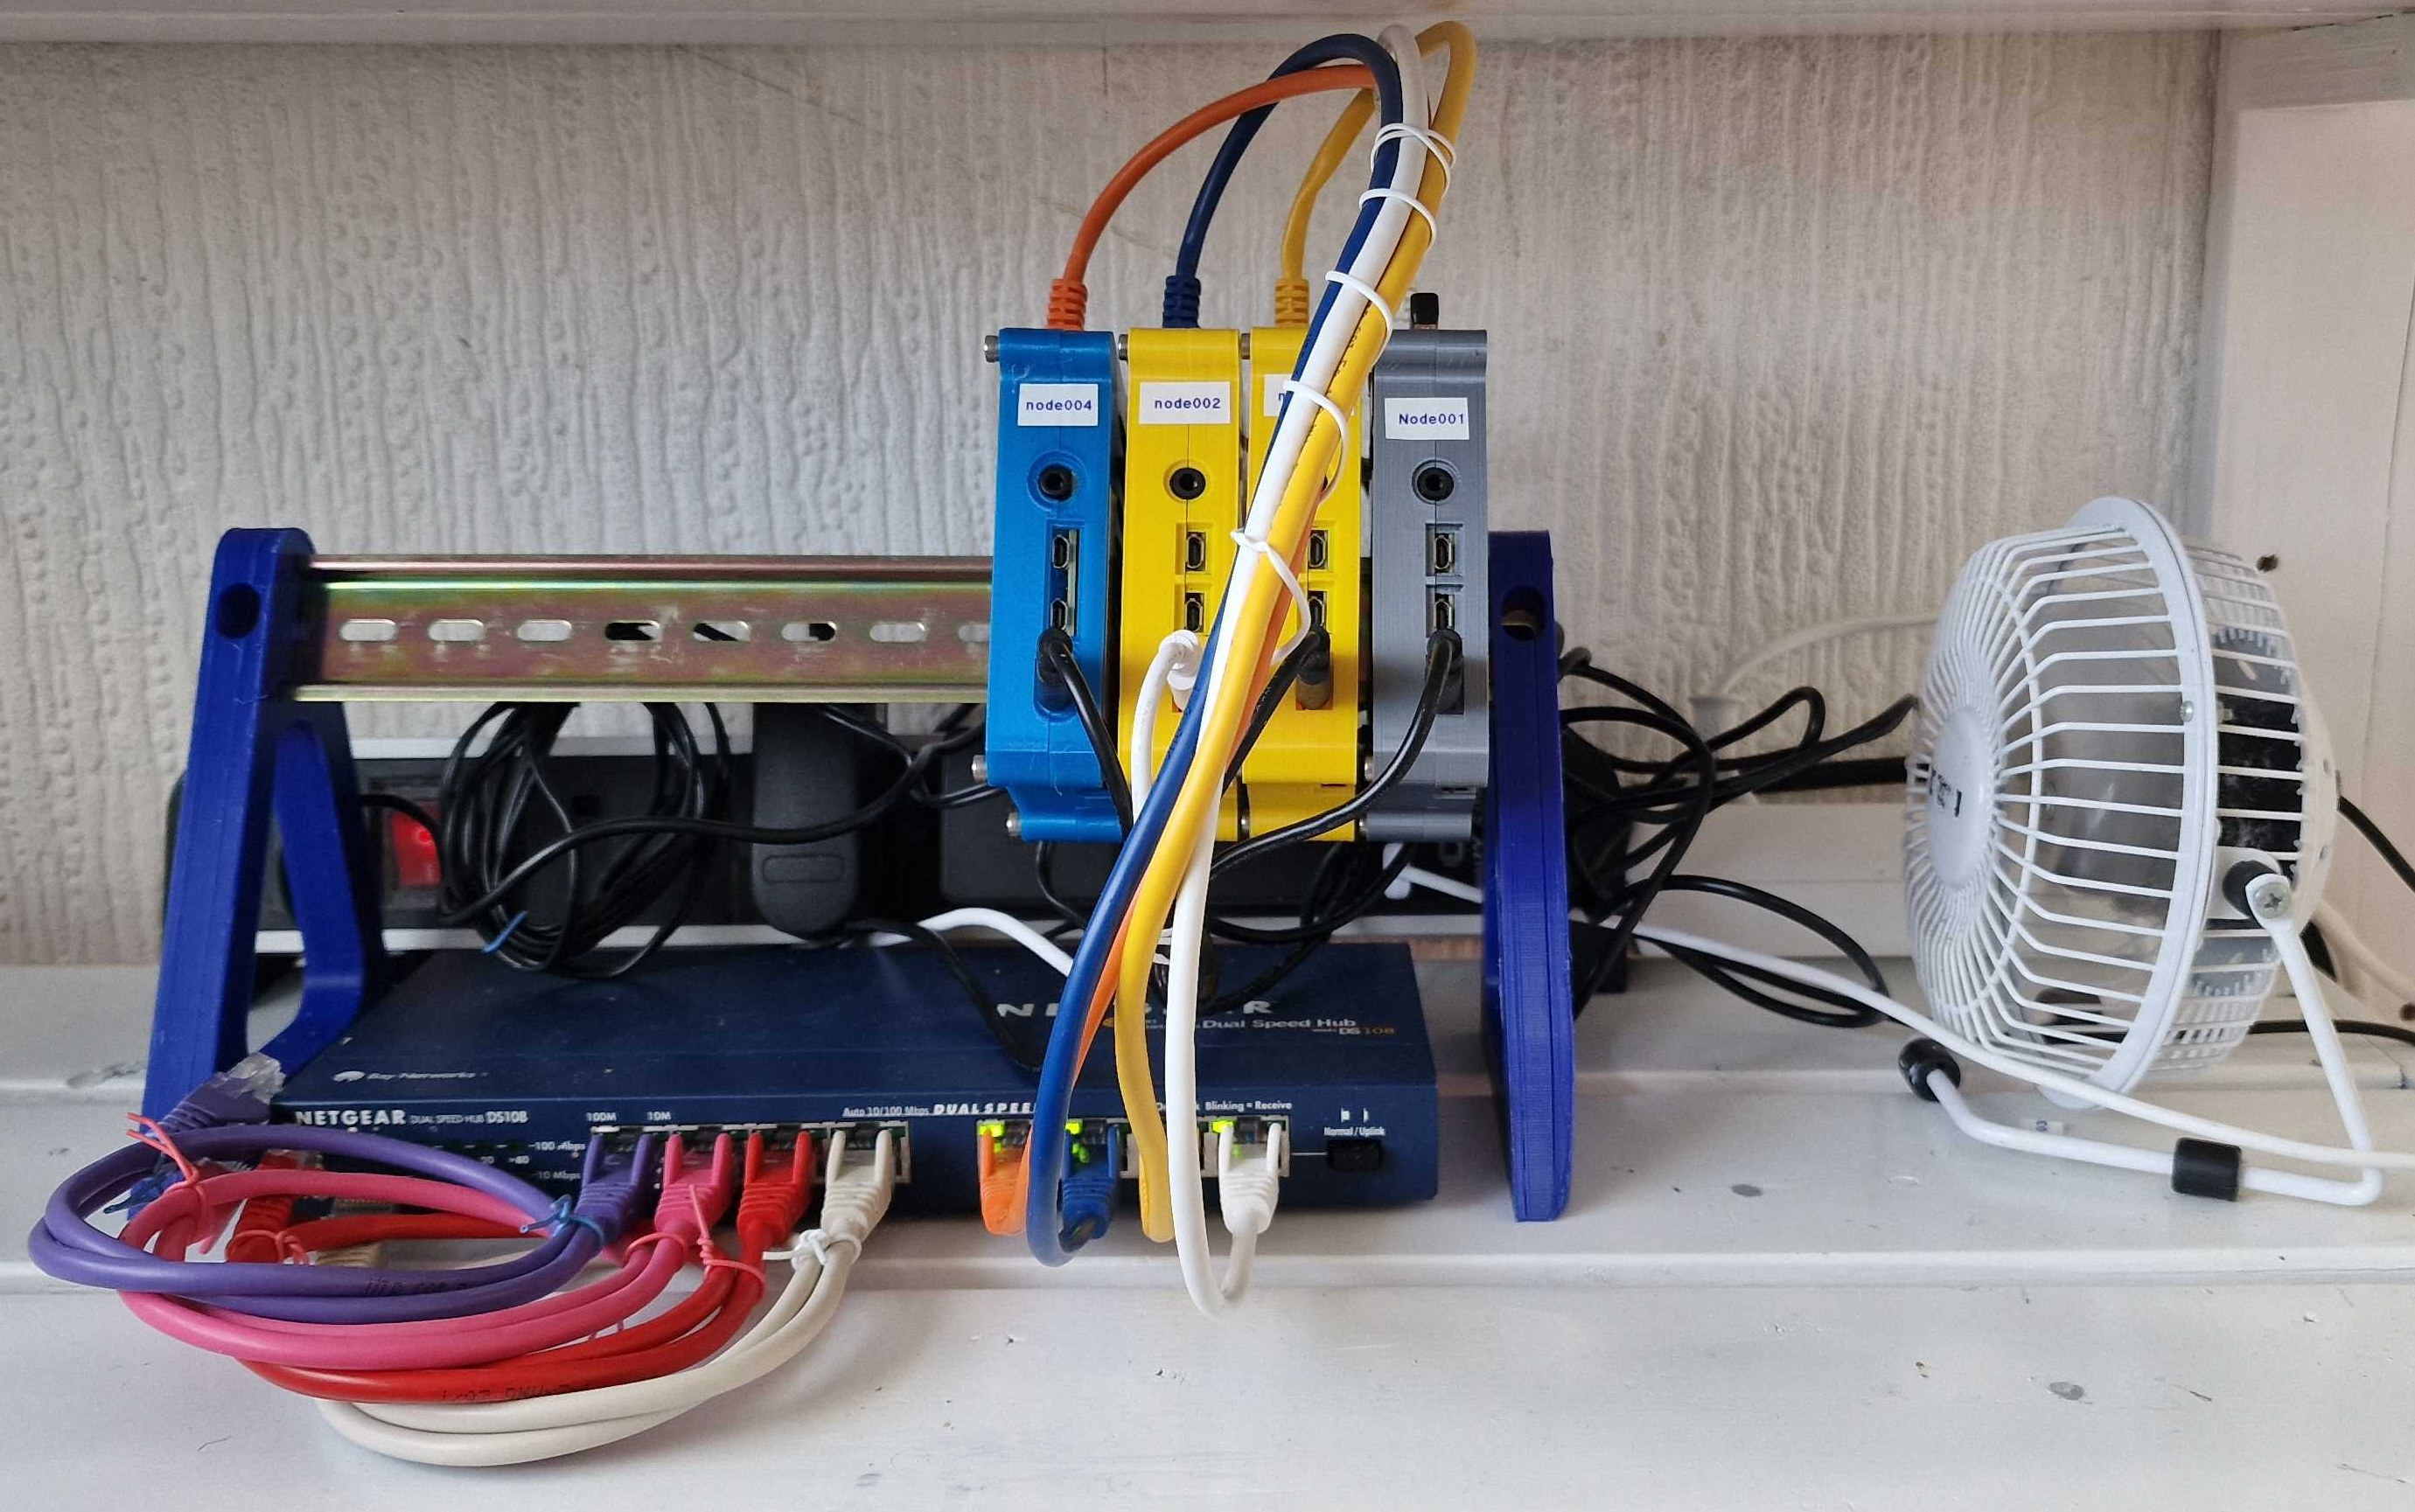
\includegraphics[width=\textwidth]{images/mini-HPC-proto1.png}
			\caption{Prototype 1}
			\label{fig:2.a}
		\end{subfigure}
		\hfill
		\begin{subfigure}[b]{0.24\textwidth}
			\centering
			\includegraphics[width=\textwidth]{images/mini-HPC-proto2.png}
			\caption{Prototype 2}
			\label{fig:2.b}
		\end{subfigure}
		\hfill
		\begin{subfigure}[b]{0.24\textwidth}
			\centering
			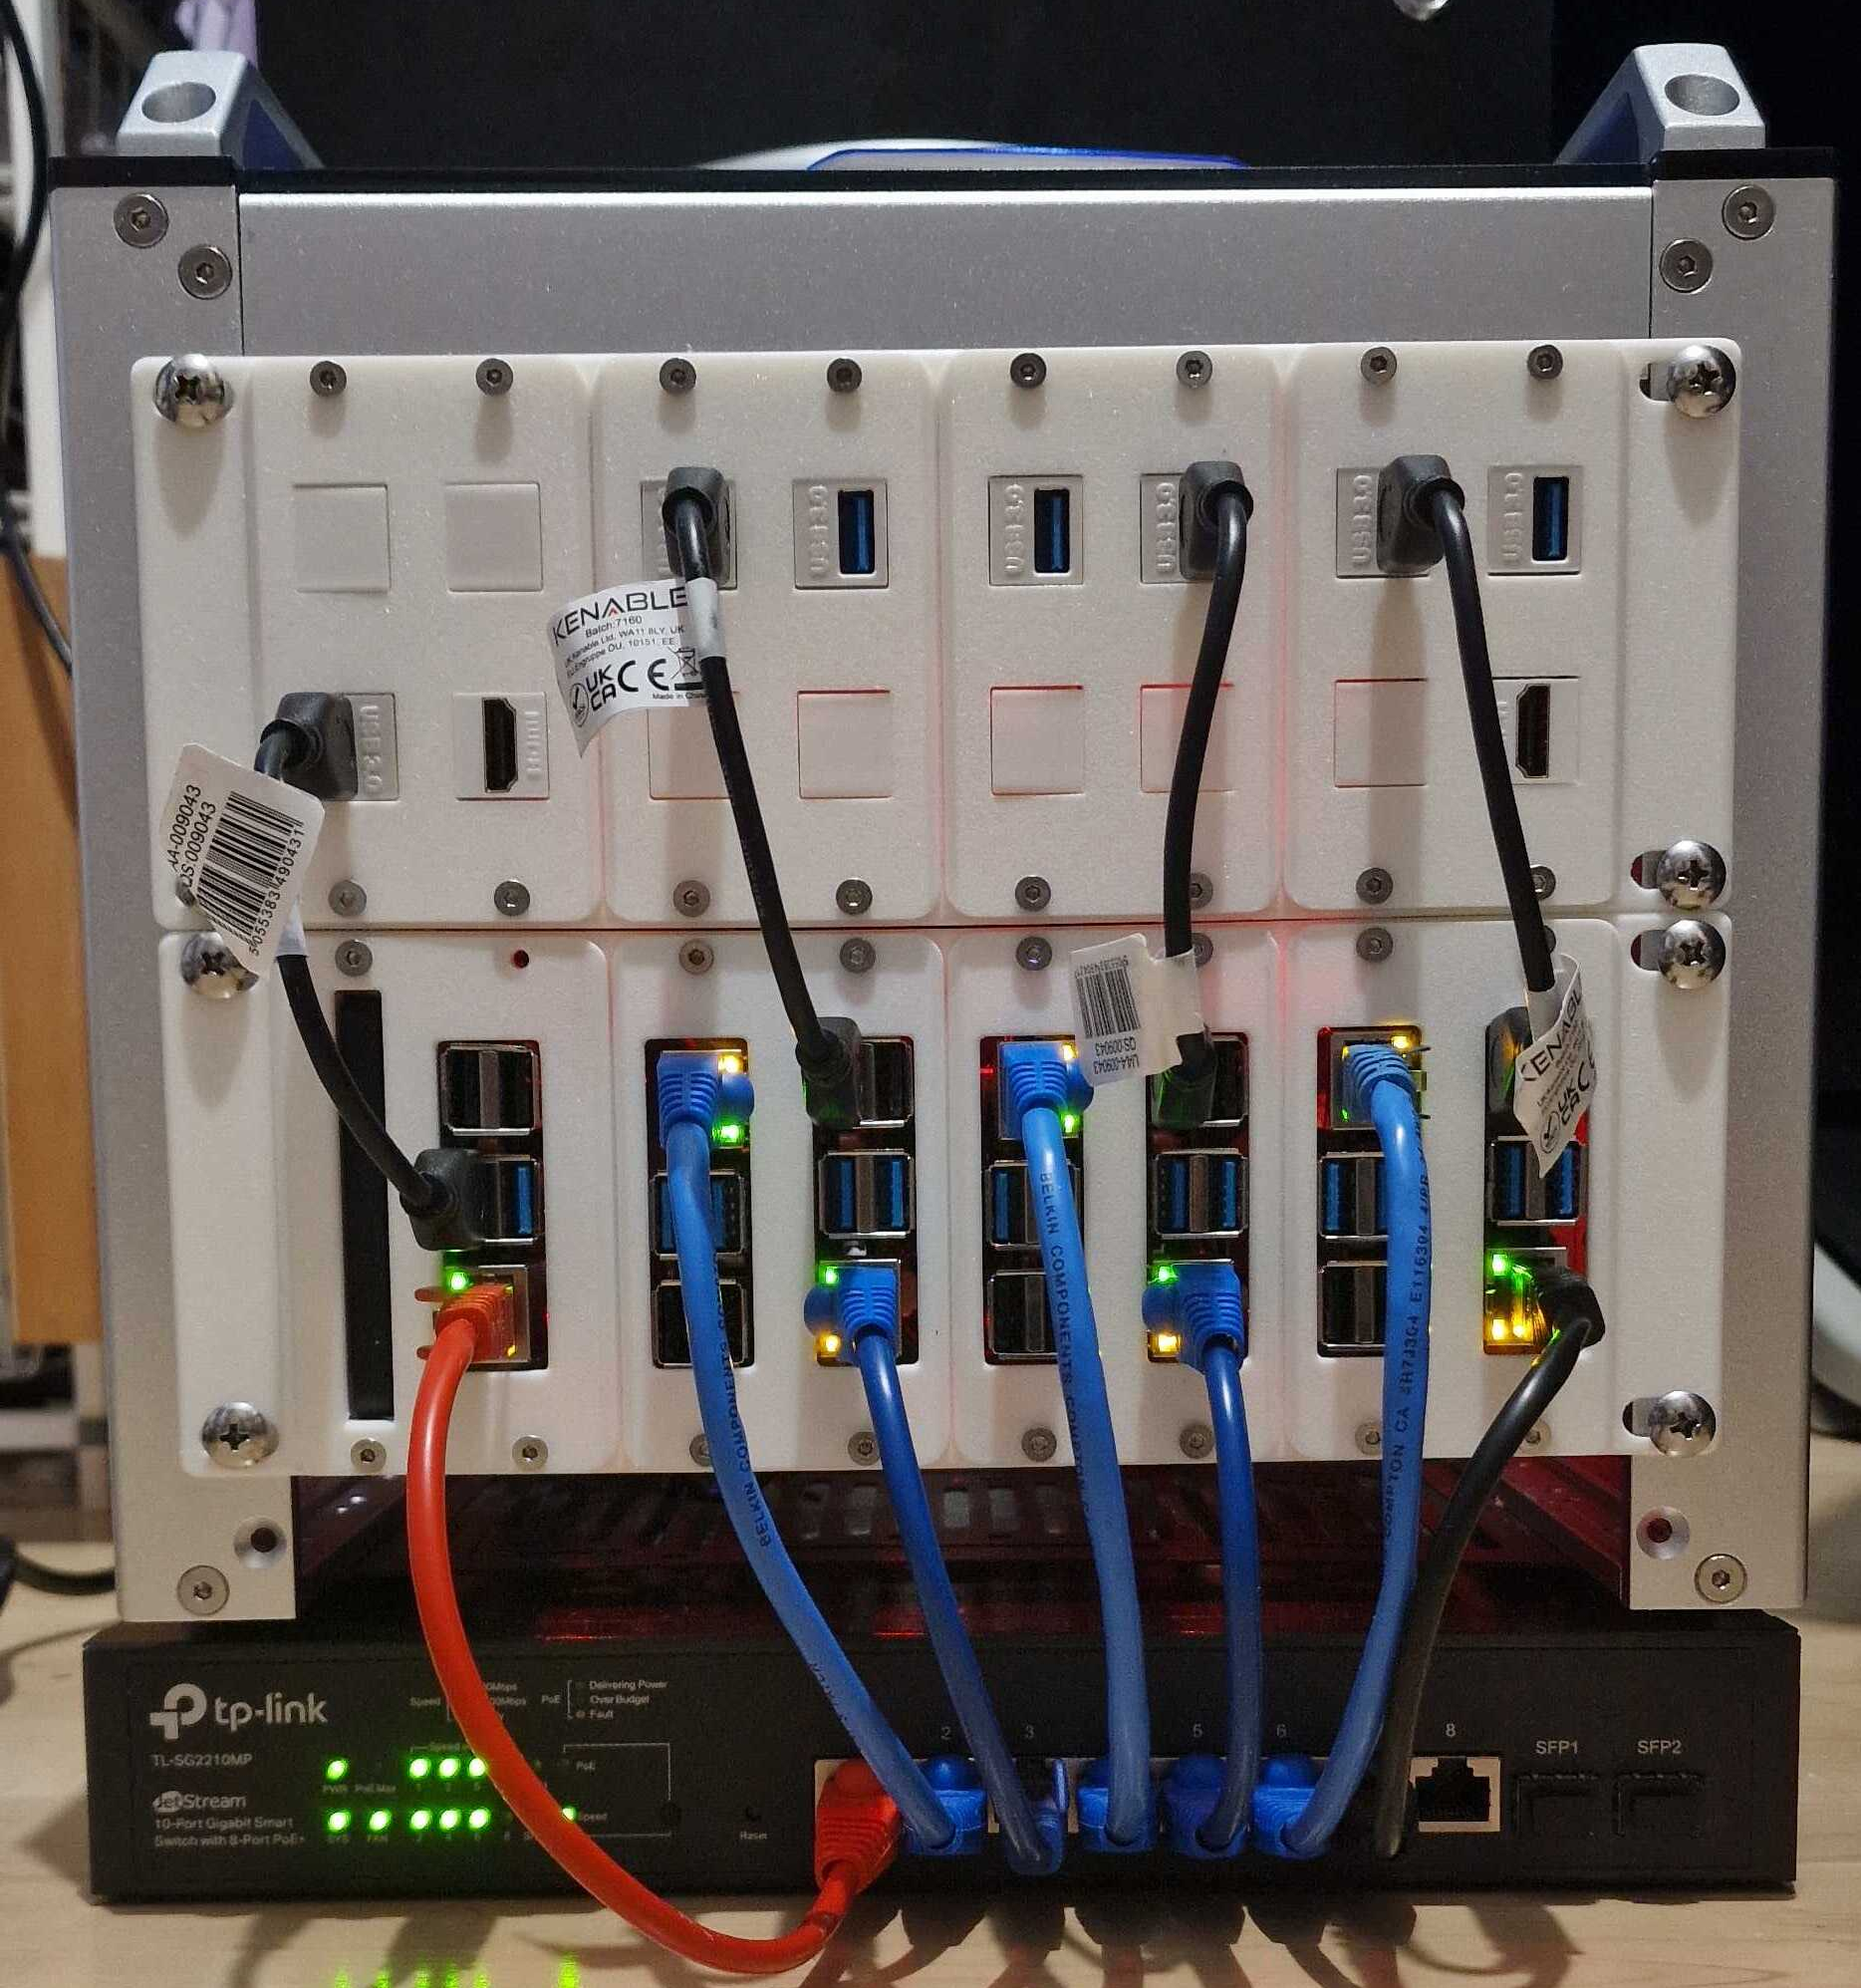
\includegraphics[width=\textwidth]{images/mini-HPC-proto3.png}
			\caption{Prototype 3 front}
			\label{fig:2.c}
		\end{subfigure}
		\hfill
		\begin{subfigure}[b]{0.24\textwidth}
			\centering
			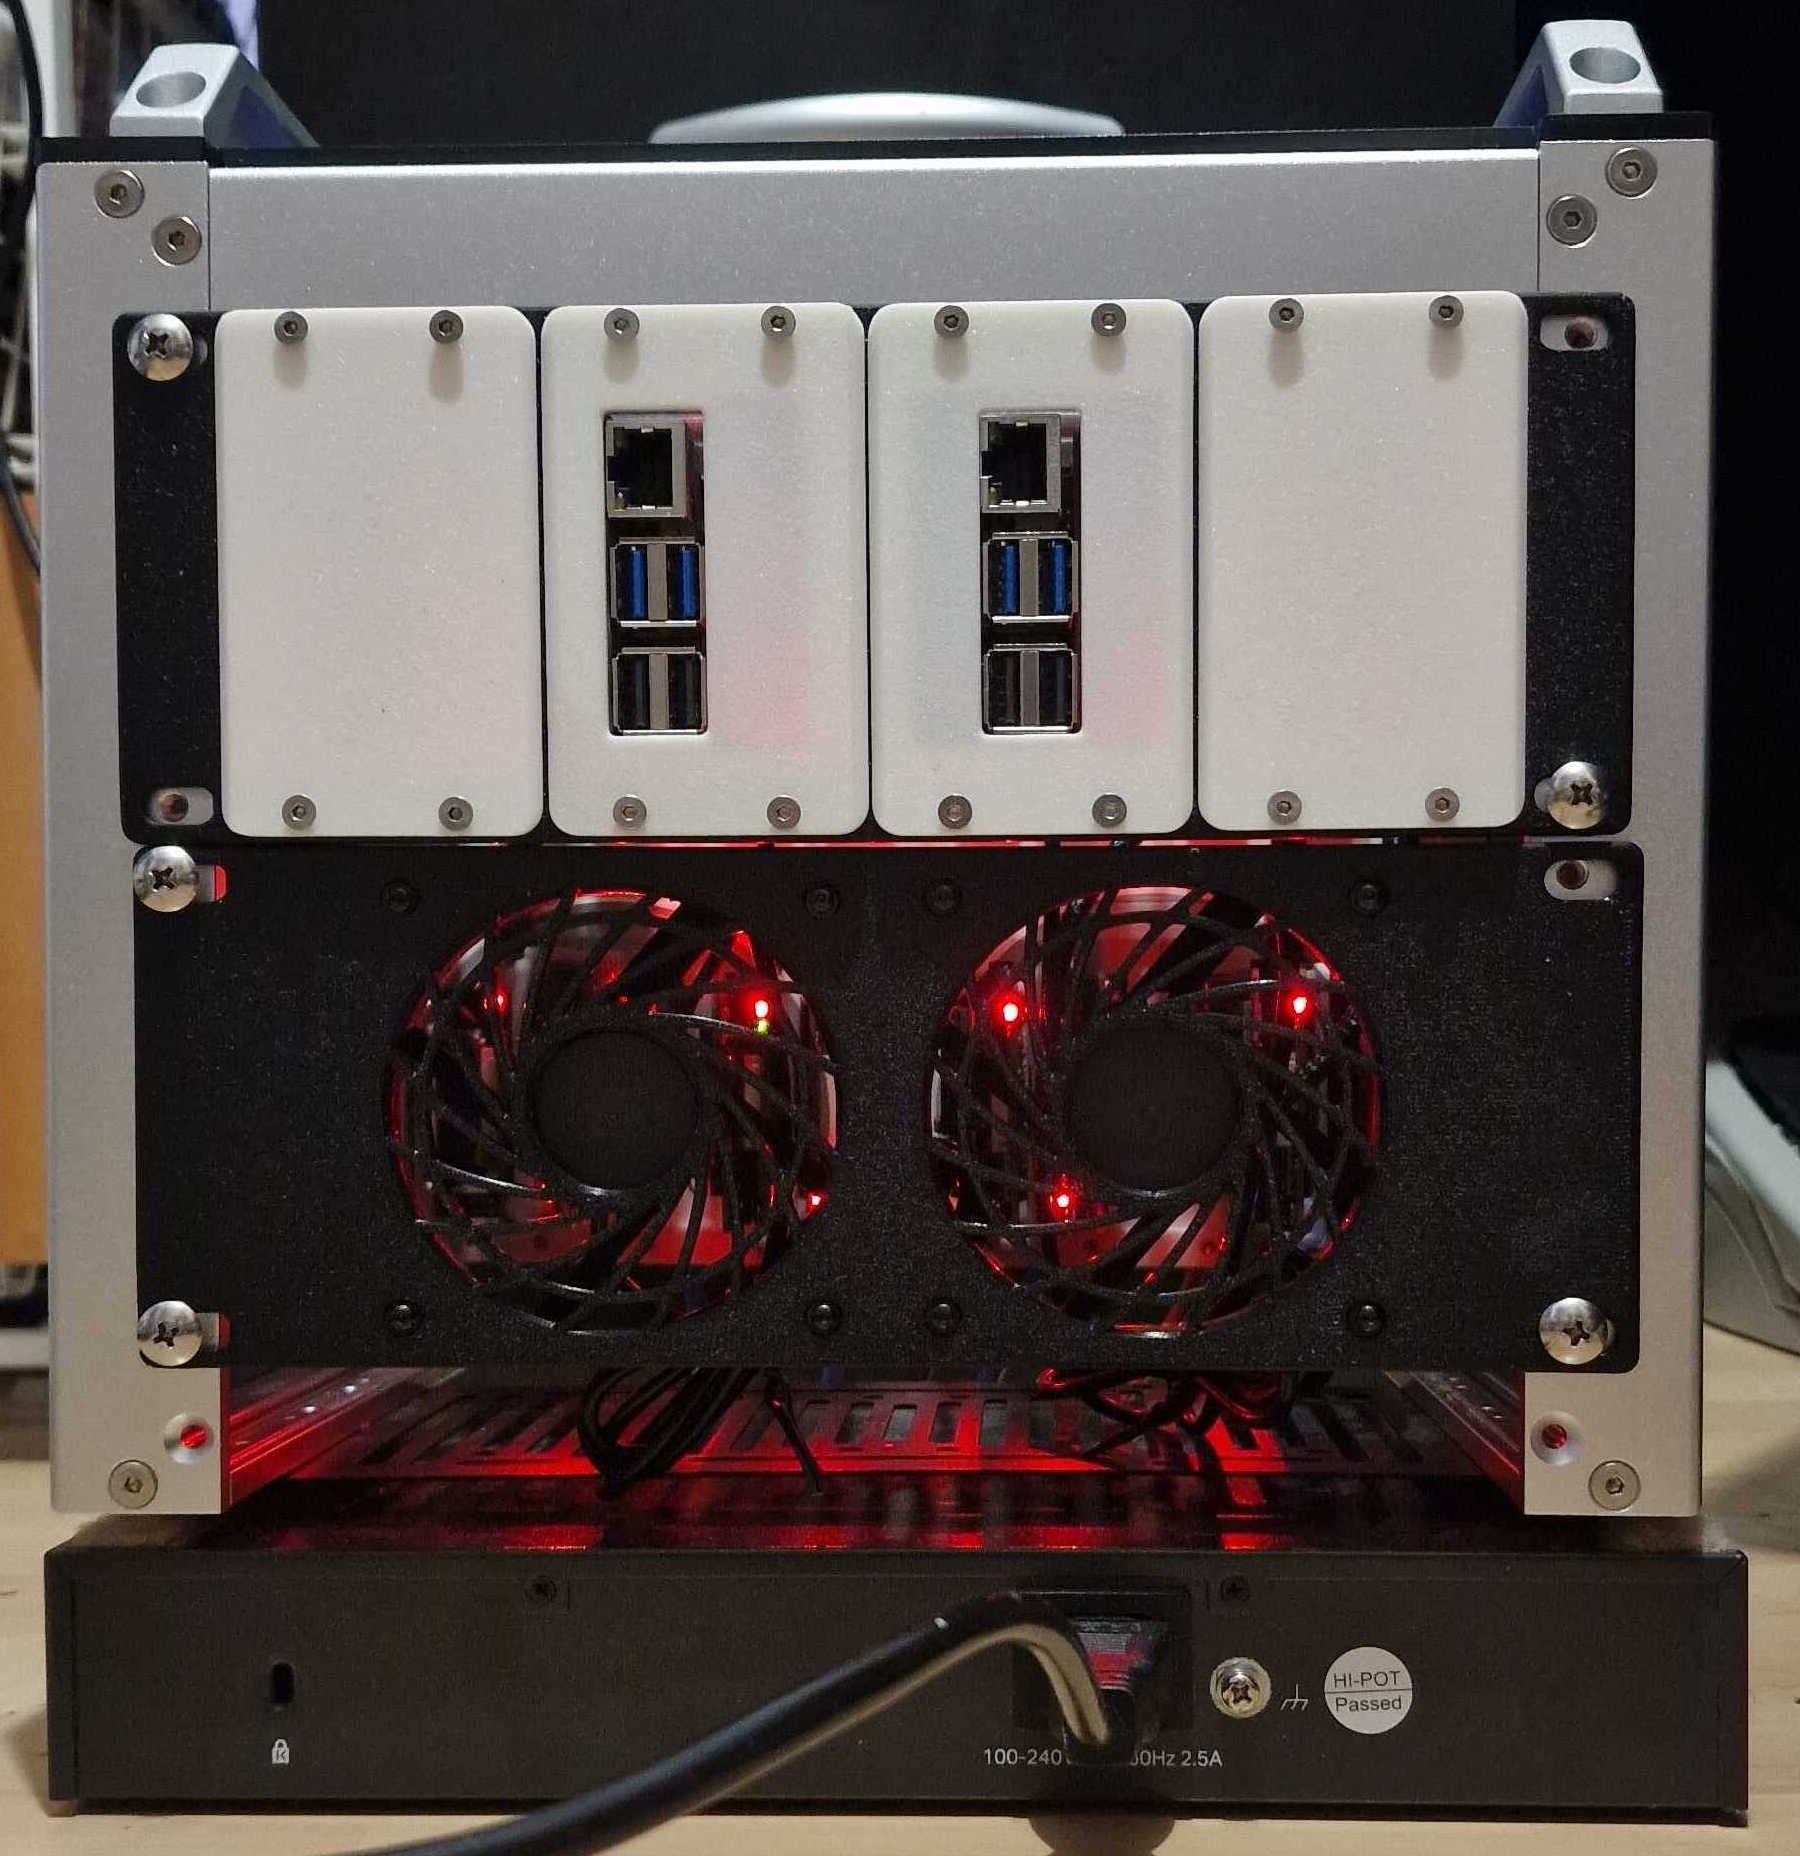
\includegraphics[width=\textwidth]{images/mini-HPC-proto3_back.png}
			\caption{Prototype 3 back}
			\label{fig:2.d}
		\end{subfigure}
		\caption{The Evolution of a miniHPC}
		\label{fig:2}
	\end{figure}
	
\end{frame}




\begin{frame}
	\frametitle{Software}
	\framesubtitle{Standard HPC Software - Typical Hardware Configuration}
	
	\begin{columns}[T]
		\begin{column}[c]{.5\textwidth}
			\begin{itemize}
				\item Slurm scheduler
				\item Shared NFS mounts
				\item lmod
				\item munge
				\item EESSI for software installations
			\end{itemize}
		\end{column}
		\begin{column}[c]{.5\textwidth}
			\centering
			
\includegraphics[width=.8\textwidth]{images/logos.png}
		\end{column}
	\end{columns}
\end{frame}


\begin{frame}
	\frametitle{The CarpentriesOffline Solution}
	\framesubtitle{Making it easier for non-specialists}
		
	\begin{columns}[c]
		\begin{column}{.65\linewidth}
			\begin{itemize}
				\item Downloadable image for booting RPi​
				\item No specialised HPC knowledge required to set up
				\item Community maintained (The Carpentries way)
				\item HPC Lesson material adapted for miniHPC
				\item Expandable with regards to hardware and software
				\item Also suitable for HPC hardware and config training
			\end{itemize}
		\end{column}
		
		\begin{column}[c]{.35\linewidth}
			\begin{figure}
				\includegraphics[width=.8\textwidth]{images/training_kit.png}
			\end{figure}
		\end{column}
	\end{columns}
 \end{frame}

\section*{Thanks}
\begin{frame}
\frametitle{}
\centering\LARGE Thank You For Listening \\
\centering\LARGE Any Questions?
	\begin{columns}[b]
		\begin{column}[b]{.35\linewidth}
			\begin{figure}
				
\includegraphics[width=.5\textwidth]{images/www.jannetta.com.png}
				\caption{www.jannetta.com}
			\end{figure}
		\end{column}
		\begin{column}[b]{.35\linewidth}
			\begin{figure}
				
\includegraphics[width=.5\textwidth]{images/carpentriesoffline.org.png}
				\caption{carpentriesoffline.org}
			\end{figure}
		\end{column}
	\end{columns}
\end{frame}



\end{document}
